\documentclass[11pt]{article}

\usepackage{amsfonts, amssymb}

\usepackage{graphicx}
\usepackage{caption}
\usepackage{tikz}
\usepackage{amsmath}





\newcommand{\chose}[2]{\left(\begin{array}{c}{#1} \\ {#2}\end{array}\right)}
\newcommand{\PI}{\textrm{PI}}
\newcommand{\BI}{\textrm{BI}}
\newcommand{\dist}{\textrm{dist}}
\renewcommand{\b}[1]{\mathbf{#1}}
\renewcommand{\c}[1]{\mathcal{#1}}
\renewcommand{\t }[1]{\mathrm{#1}}
\newcommand{\bb}[1]{\mathbb{#1}}
\newcommand{\bR}{\bb R}
\renewcommand{\L}{\c L}
\newcommand{\eqop}{=}
\renewcommand{\phi}{\varphi}
\tikzstyle{no1}=[circle, draw, fill = yellow!65!green, inner sep = .1 cm]
\tikzstyle{no2}=[circle, draw, fill = yellow!95!green]
\tikzstyle{no3}=[circle, draw, fill = yellow!95!green, minimum size= .35 in]
\tikzstyle{no4}=[circle, draw, fill = yellow!65!green, minimum size= .35 in]
\renewcommand{\rmdefault}{ppl} %Change the font
\begin{document}

%PIC 1
\begin{center}
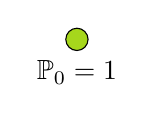
\begin{tikzpicture}[level distance=2.5cm]
  \tikzstyle{level 1}=[sibling distance=3cm];
  \node[no1, label= south:{$\bb{P}_0\eqop 1$}] (root) {};
\end{tikzpicture}
\\
$$$$
%PIC 2
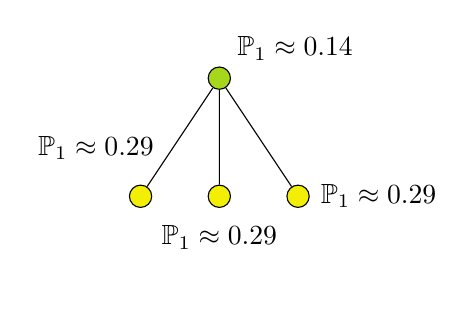
\begin{tikzpicture}[level distance=1.5cm]
  \tikzstyle{level 1}=[sibling distance=1cm];
  \node[no1, label=north east:$\bb{P}_1 \approx 0. 14$] (root) {}
   [no1, ]
     child {node[no2, label={[label distance=-0.2cm]170:$\bb{P}_1 \approx 0.29$ }] {}
      }
child  {node [no2, label=   {[label distance=-.5cm]270 :$\bb{P}_1 \approx 0.29$}]{}
     }
  child  {node [no2, label={[label distance=0cm]0:$ \bb{P}_1 \approx 0.29$}]{}
           };
\end{tikzpicture}


%PIC 3
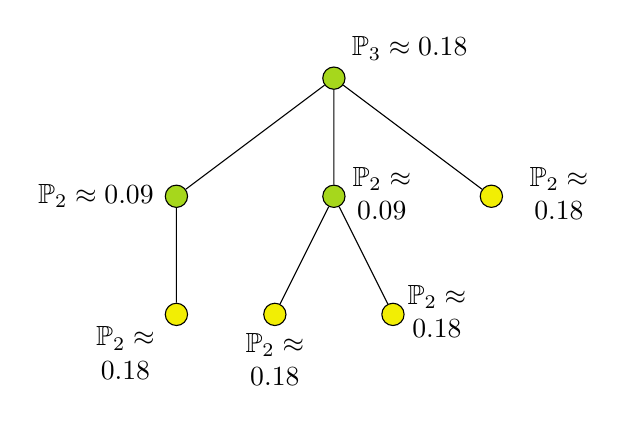
\begin{tikzpicture}[level distance=1.5cm]
  \tikzstyle{level 1}=[sibling distance=2cm];
  \tikzstyle{level 2}=[sibling distance=1.5cm];
  \node[no1, label=north east:$ \bb{P}_3 \approx 0. {18}$] (root) {}
   [no1, ]
     child {node[no1, label= west:$\bb{P}_2 \approx 0. {09}$ ] {}
       child  {  node[no2, label = {[label distance=0 cm]190 :$\begin{matrix} \bb{P}_2\approx\\  0.{18}\end{matrix}$}]{}
		}
      }
child  {node [no1, label={[label distance=-.25cm]0:$\begin{matrix}\bb{P}_2 \approx\\  0. {09}\end{matrix}$}]{}
       child {node[no2, label=   {[label distance=-0.25cm]-90 :$\begin{matrix}  \bb{P}_2 \approx\\ 0.{18}\end{matrix}$}] {}}
       child {node [no2, label=  {[label distance=-.3cm]0: $\begin{matrix} \bb{P}_2 \approx\\ 0.{18}\end{matrix}$}]{}}
     }
  child  {node [no2, label= {[label distance=0cm]0:$\begin{matrix}\bb{P}_2 \approx\\ 0.{18}\end{matrix}$}]{}
           };
\end{tikzpicture}
\end{center}
\end{document}

